\documentclass[border=8pt,tikz]{standalone}
% https://tex.stackexchange.com/questions/733659/how-to-tune-the-function-of-line-to-operation-and-in-tikz
\usetikzlibrary{positioning,ext.paths.ortho}
\begin{document}
    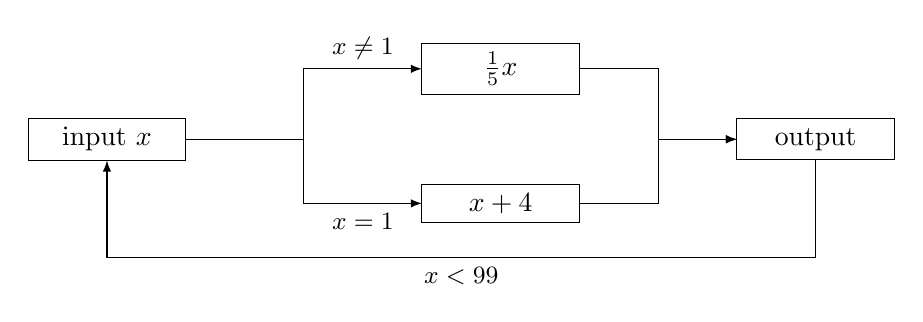
\begin{tikzpicture}[
        cap = round,
        rectangle/.style = {
            draw,outer sep=0pt,
            minimum width=2cm},
        arr/.style = {-latex},
        lib/.style = {pos=#1,font=\small},
]
        \node[rectangle] (A) {input $x$};
        \node[rectangle] (C) [above right=.3 and 3 of A] {$\frac15x$};
        \node[rectangle] (D) [below right=.3 and 3 of A] {$x+4$};
        \node[rectangle] (F) [right=7 of A] {output};
        \draw [arr] (A) -|- (C) node[lib=0.875,above]{$x\ne1$};
        \draw [arr] (A) -|- (D) node[lib=0.875,below]{$x=1$};
        \draw [arr] (C) -|- (F);
        \draw [arr] (D) -|- (F);
        \draw [arr] (F) --++(0,-1.5cm) -| (A) node[lib=0.25,below]{$x<99$};     
    \end{tikzpicture} 
\end{document}